
%TODO
%PDR opisywany behawioralnie, nie wdawać się w szczegóły - pominąć dokładny opis struktur danych.
%Do obsługi dużych klatek (nadpróbkowanie 16x) należy przeprogramować zarówno VDMA jak i ADC interface. Trzeba podzielić dużą klatkę na mniejsze bo inaczej nie zmieści się w VDMA.

%Określić sposób ładowania systemów operacyjnych oraz sposób uruchamiania programów - w jaki sposób obejść problem z uruchamianiem cachu
%Dopracyzować poszczególne stuktury danych, aby można było oszacować ile cała impreza zajmie pamięci
%Doprecyzować listę i sposób kodowania rozkazów
%Doprecyzować listę, sposób kodowana i ew. rodzaj generowanych odpowiedzi
%Dokończyć mapę pamięci
%W jaki sposób ma być zrealizowana obsługa błędów na poziomie FreeRTOSa?
%Czy opisy sposobu testowania umieścić w oddzielnych dokumentach dotyczący poszczególnych modułów kamery?
%Jakie powinny być długości danych (np. timestampy? - 64 bit?) Timestamp: 32bit - sekundy 32bit- nanosekundy
%Opracować z Konradem specyfikację danych dla migawki
%Opracować strukturę danych dla peltiera
%Wyzwalanie triggera odbywać się będzie na linuksie


%TODO
%PYTANIA I PROBLEMY
% - Jest problem z DMA dla nadpróbkowania 16x - kontroler nie obsługuje tak dużych ramek obrazu (rozmiar podaje się w bajtach)
% - Jak zrealizujemy oknowanie sygnału z CCD?

%Do Pawła
% - Jak będzie wyglądał interfejs pomiędzy Epic a serwerem sterującym kamerą?
% - Czy diagnostyka będzie przeprowadzana przez Epica?
% - Ja robię diagnostykę na FreeRTOSie, Paweł na linuksie

\subsection{Introduction}

%\todo[inline, caption={IPC Polling/Interrupt}]{Czy podjęta została ostateczna decyzja odnośnie implementacji IPC na pollingu a nie przerwaniach? Można wykorzystać jedno przerwanie z GICa i jechać na nim, może to być lepsze rozwiązanie, na początku tylko więcej zachodu. Można sprawdzić to: http://henryomd.blogspot.com/2015/02/zynq-inter-process-interrupts.html  /PZi}

This section describes proposed interprocessor communication architecture to be used in Neostel camera. As it was decided beforehand that camera APU will operate in AMP mode running two independent operating systems - Linux and FreeRTOS, current section limits it's scope to those OSes and ARM Cortex A9 dual core architecture (Zynq - 7000). \\
System utilizes bidirectional communication based on message queues. Communication occurs between process running on one APU core and task running on the other. Process running on Linux OS issues commands, while FreeRTOS task reads and executes commands. For every command issued by the master there is one acknowledgement response generated by the slave. Commands are issued and executed sequentially, one at a time. Before next command can be issued, previous has to finish. Additionally FreeRTOS can send asynchronous event messages such as unexpected error to Linux, without being polled first. Both commands and responses are sent through their respective FIFO message queues implemented in shared memory regions.

\vspace{\baselineskip}
Key assumptions:
\begin{itemize}
\item asynchronous communication based on polling - no interprocessor interrupts (no need to write specialized linux driver)
\item master - slave architecture
\item commands, responses and data separation - commands and responses in FIFOs, data in their respective shared memory regions
\item sequential commands execution - one command at time
\item every command generates response
\item slave can send asynchronous event messages to the master
\item address table known at compilation time
\item known and constant length data structures
\item no command execution time guarantees
\item camera server API functions blocking with timeout
\end{itemize}

\begin{figure}[H]
\centering
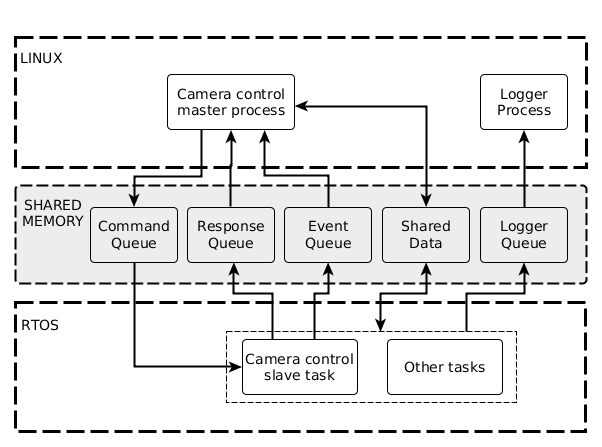
\includegraphics[width=0.7\textwidth]{pict/ipc.png}
\caption{IPC architecture}
\label{fig:ipc_arch}
\end{figure}


\subsection{Camera messages}
Current sections presents draft of IPC messages structure. Presented command and responses lists are not final yet and can be changed during later development phases.

\subsubsection{Commands list}

\begin{itemize}
\item write\_cfg \hfill \\
Writes configuration to camera buffer register. Configuration is applied to camera when ARM command is received.
\item read\_cfg \hfill \\ 
Reads configuration from camera buffer register.
\item test\_shutter \hfill \\ 
Carries out test of shutter subsystem.
\item test\_adc\_interface \hfill \\
Carries out test of ADC interface.
\item test\_peltier \hfill \\
Carries out test of peltier cooling subsystem.
\item get\_camera\_state \hfill \\
Queries for state in which camera currently is in.
\end{itemize}

\subsubsection{Commands format}
Each command is encoded as 8-bit (1 byte) value.

\begin{table}[H]
\begin{center}
    \begin{tabular}{ | l |}
    \hline
    Command code (1 byte)\\ \hline
    \end{tabular}
    \end{center}
    \caption{Command format}
	\label{table:command_format}
\end{table}

\subsubsection{Commands coding table}

\begin{table}[H]
\begin{center}
    \begin{tabular}{ | l || l |}
    \hline
    Command 				& Opcode 	\\ \hline
	write\_cfg 			& 0 	\\ \hline
	read\_cfg			& 1 	\\ \hline
	test\_shutter		& 2 	\\ \hline
	test\_adc\_interface	& 3 	\\ \hline
	test\_peliter		& 4 	\\ \hline
	get\_camera\_state		& 5 	\\ \hline
    \end{tabular}
    \end{center}
    \caption{Commands coding table}
	\label{table:command_enc_table1}
\end{table}

\subsubsection{Responses list}
All responses carry response value (rval). In cases, when command can fail, response value shall be treated as error code - rval = 0 : command succeeded, rval > 0 : command failed, error code.

\begin{itemize}
\item write\_cfg\_acq \hfill \\
Write configuration response.
\item read\_cfg\_acq \hfill \\ 
Read configuration response.
\item test\_shutter\_acq \hfill \\ 
Shutter subsystem test response.
\item test\_adc\_interface\_acq \hfill \\ 
ADC interface subsystem test response.
\item test\_peltier\_acq \hfill \\
Peltier cooling subsystem test response.
\item get\_camera\_state\_acq \hfill \\
Returns state in which camera currently is in.
\end{itemize}

\subsubsection{Response format}
Response has additional byte-size field which contains response code.

\begin{table}[H]
\begin{center}
    \begin{tabular}{ | l | l |}
    \hline
    Response code (1 byte) & Response value (1 byte)\\ \hline
    \end{tabular}
    \end{center}
    \caption{Response format}
	\label{table:response_format1}
\end{table}

\subsubsection{Responses coding table}

\begin{table}[H]
\begin{center}
    \begin{tabular}{ | l || l  |}
    \hline
    Response 			& Opcode 	\\ \hline
	write\_cfg\_acq 		& 0 	\\ \hline
	read\_cfg\_acq 			& 1 	\\ \hline
	test\_acq 				& 2 	\\ \hline
	camera\_state\_acq		& 3 	\\ \hline
    \end{tabular}
    \end{center}
    \caption{Responses coding table}
	\label{table:command_enc_table2}
\end{table}

\subsubsection{Event messages}

Event message has similar format as response message - it consists of two fields: event code and event value. Important difference is that event message can be sent by RTOS asynchronously without being queried by Linux first.

\begin{table}[H]
\begin{center}
    \begin{tabular}{ | l | l |}
    \hline
    Event code (1 byte) & Event value (1 byte)\\ \hline
    \end{tabular}
    \end{center}
    \caption{Event format}
	\label{table:response_format2}
\end{table}

\begin{table}[H]
\begin{center}
    \begin{tabular}{ | l || l  |}
    \hline
    Event 			& Event code 	\\ \hline
	shutter0 mechanical problem			& 0 	\\ \hline
	shutter0 overheat					& 1 	\\ \hline
	shutter0 unknown error				& 2 	\\ \hline
	shutter0 shutter emergency shutdown & 3 	\\ \hline
	shutter1 shutter emergency shutdown & 4 	\\ \hline
	shutter1 mechanical problem			& 5 	\\ \hline
	shutter1 overheat					& 6 	\\ \hline
	shutter1 unknown error				& 7 	\\ \hline
	shutter0 action request				& 8 	\\ \hline
	shutter1 action request				& 9 	\\ \hline
	peltier failure						& 10 	\\ \hline
	picture ready						& 11 	\\ \hline
	arm\_acq				& 12 	\\ \hline
	trig\_acq 			& 13 	\\ \hline
	
    \end{tabular}
    \end{center}
    \caption{Event coding table}
	\label{table:event_enc_table}
\end{table}

\subsection{Interprocessor synchronization and mutual exclusion mechanism}
Due to relatively narrow array of tasks running between both operating systems it was decided that simple spin lock should suffice to provide synchronization and mutual exclusion. Spin lock is implemented utilizing hardware atomic instructions on ARM architecture.

\subsubsection{Spin lock implementation}
Spin lock is implemented in shared memory region. \emph{lock()} operation is realized as GCC built-in atomic function \emph{\_\_sync\_lock\_test\_and\_set(sem,1)} while \emph{unlock()} function is implemented using \emph{\_\_sync\_lock\_release(sem)}, where \emph{sem} is address in shared memory.

\subsubsection{Spin lock initialization}
It was decided, that spin lock initial value should be set by Linux process, before FreeRTOS task starts and is able to acquire it.

\subsubsection{FIFO queue}

Key assumptions:
\begin{itemize}
\item one producer one consumer 
\item synchronized by spinlock
\item constant depth
\item constant element size
\end{itemize}

\subsubsection{Shared data structure}
\label{fifofmt}
%FIXED
%\todo[inline, caption={FIFO opis}]{FIFO ze strukturą z magicznymi wskaźnikami do pamięci? taki zapis nie jest jednoznaczny wg mnie. W przypadku podawania adresu w pamięci poprzez adres linearyzowany z MMU to już nie jest wskaźnik tylko normalna liczba (nie licząc tego, że wskaźnik zawsze jest liczbą). Taki zapis powoduje, że przekazuje się adres w jeszcze innej przestrzeni, Linuxowej, która niekoniecznie musi się zbiegać z tą procesora. /PZi }


Every IPC FIFO queue used in project uses data structure presented on listing \ref{lst:queue_head}. Data structure consists of five fields, of which first three are kept in shared memory. \emph{buf} points to memory region containing queue body (elements array). \emph{head} and \emph{tail} point to head and tail of the queue respectively. \emph{depth} contains maximum number of elements in the queue while \emph{size} keeps size (in bytes) of a single element. All three pointers ultimately point to the same places in memory both in Linux and in RTOS, but are not the same - in case of Linux these pointers represent virtual addresses mapped to the physical ones while in RTOS these pointers represent physical addresses directly.

\begin{lstlisting}[caption={FIFO header data structure} ,language=C , captionpos=b, label=lst:queue_head]
typedef struct
{
     char* buf;
     uint32_t* head;
     uint32_t* tail;
     uint32_t depth;
     uint32_t size;
} fifo_t;

\end{lstlisting}

\subsubsection{Command queue}
Command FIFO queue consists of header and FIFO body, all stored in IPC shared memory. FIFO header format \ref{fifofmt} is the same as for any other IPC FIFO used in the project. FIFO body consists of data array of 1-byte commands. Because of previous assumption that next command can only be issued after previous has been finished, minimal FIFO length should be 1.

\subsubsection{Response queue}
Response FIFO queue has exactly the same format as command FIFO with exception that responses (queue elements) are 2-byte long.

\subsection{FreeRTOS output logging}
It was decided that FreeRTOS output will be logged independently of Linux output. Established architecture imposes method of logging similar to the other IPC mechanisms - sending data to Linux process through shared FIFO. Linux process then writes received log lines as a text file to selected medium, for example memory or SD Card.

\subsubsection{Log format}
Log line consists of timestamp and text information.

\subsubsection{Logger FIFO}
Queue element size was decided to be of 256 byte length: 255 characters + terminating 0. Queue depth shall be long enough to prevent FIFO fillup during intense logging events i.e. during tests and debugging. Initially it was decided to be 128.

\subsection{IPC tasks and processes}
There are 2 tasks communicating with each other - one for either operating system. On Linux it is implemented as separate process and called Camera Command Master. On FreeRTOS it is implemented as separate FreeRTOS task and called Camera Command Slave. Additionally there is separate logger process on Linux, gathering output from FreeRTOS tasks and putting it into log text file.

\subsection{Data formats definition}

\subsubsection{Introduction}

\subsubsection{Groups of data interchanged between OSes}
Data gathered by the processing system can be grouped into following 3 distinct categories:

\begin{itemize}
\item Sensors (temperature, humidity, power supply voltage etc.)
\item Image frame: image data, shutter position and timestamps, peltier flags
\item Configuration data
%\item Debug data (for example IP Cores debug)
\end{itemize}

Each category contains different kind of data, which is collected at distinct intervals. Sensors data is collected and monitored continuously with interval of about a second in diagnostic purposes. Image data is collected only at request, after prior arming and releasing a trigger. Configuration data is only changed and read on user request. During camera start-up process default configuration is loaded. 
%Debug data is available on request in case of registering error.

\subsubsection{Sensors data format}
Sensors data are logged by RTOS into triple buffer in shared memory. Most recently logged sensor frame address is available through camera server API. All sensors measurements are converted by RTOS from their native formats and stored in 32-bit float format. Physical quantities measured are: temperature, humidity, acceleration, coolant volumetric flow and power supply voltage.

\begin{itemize}
\item Temperature - ${}^{\circ}\mathrm{C}$
\item Humidity (relative) - unitless (\%)
\item Acceleration - ${m} \over {s^2}$
\item Coolant Volumetric Flow Rate - lpm (${dm^{3}} \over {min}$)
\item Voltage - V
\end{itemize}

\subsubsection{Frame data format}
Image data frame consists of image data size,raw image data, peltier activity flags (one per line of picture), shutter data and trigger time stamp.

%\begin{figure}[H]
%\centering
%\includesvg[width=0.3\textwidth, svgpath = pict_ipc/]{frame_format}
%\caption{Image data frame format}
%\end{figure}

\begin{figure}[H]
\centering
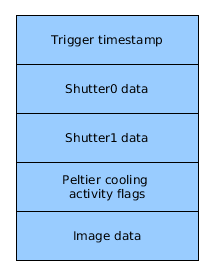
\includegraphics[width=0.3\textwidth]{pict_ipc/frame_format.png}
\caption{Image data frame format}
\label{fig:frame_format}
\end{figure}


\begin{description}
\item \textbf{Image data} \hfill \\
Nominal size of CCD sensor is 4096x4096 pixels. Each pixel is sampled with 16-bit resolution and consists of two samples: one of video level and another of black level. This gives in total 4096x4096x2x2 = 64MB of data. Due to high SNR requirements each pixel has to be oversampled. Two agreed oversampling factors are 4x and 16x. Taking into account oversampling, frame sizes are respectively 256MB and 1024MB. In order to speed up processing and save memory, samples are processed and decimated on the fly in FPGA. Resulting image frame written to memory has size of 4096x4096x2 = 32MB. In case of binning or any other picture size changing operation enabled frame size stays the same - only less space in image data field is used.

\item \textbf{CCD cooling activity flags} \hfill \\
For debug purposes, CCD cooling system status information is written along with picture data. For each line of picture there is one bit of CCD cooling system activity information. If cooling system was active during readout of this particular line, then this bit is set to 1. CCD cooling status information takes 4096/8=512 bytes of data.

\item \textbf{Shutter data format} \hfill \\
Shutter data is formatted as table containing shutter position samples, taken in constant interval from position sensor. Additionally shutter data frame contains shutter acceleration information and timestamps. Shutter opening and closing signal assert is timestamped. In order to obtain shutter opening time/position profile, internal shutter counter is utilized. Counter starts when shutter control line is asserted and counts until shutter finishes operation. Because line assertion is timestamped, absolute time can be calculated from counter values.
\end{description}

\begin{figure}[H]
\centering
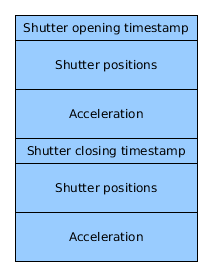
\includegraphics[width=0.3\textwidth]{pict_ipc/shutter_format.png}
\caption{Shutter data format}
\label{fig:shutter_format}
\end{figure}

\todo[inline, caption={picture update}]{Obrazek jest mylacy, co to jest Acceleration. KZg}

\subsubsection{Configuration data format}

\begin{itemize}
\item pattern generator program
\item pattern generator program size (16 bit) (in no. of instructions)
\item pattern generator max. program size: 4096 instructions (each instruction 128 bit long)
\item exposure time (in milliseconds, uint32\_t) (at least 300s needed)
\item readout mode (oversampling factor)
\item binning mode (4 combinations - no binning ,2x horizontal, 2x vertical, both)
\item windowing mode on/off
\item window coordinates
\item peltier cooling config parameters
\item AFE parameters
\item shutter configuration
\item temperature monitor parameters
\item camera hardware sensors readout period
%\item MPP mode on/off
\end{itemize}

%\begin{lstlisting}[caption={Configuration data format} ,language=C , captionpos=b, label=lst:config]
%struct
%{
%	uint32_t* pattern_gen_prog;
%	uint32_t prog_len; //max 4096 instructions?
%	uint32_t exp_t;
%	uint32_t rd_mode;
%	uint32_t trig_t; // trigger release time: same format as timestamps
%
%} neocam_config_t;
%\end{lstlisting}

%\subsubsection{Debug data format}
%
%\textcolor{red}{Debug data contains auxiliary debug information, apart from those contained in FreeRTOS log. For example this frame may contain context information in case of error.}

%\begin{figure}[H]
%\centering
%\includegraphics[width=0.7\textwidth]{picture/unnamed0.svg}
%\caption{opis}
%\label{fig:panex}
%\end{figure}

%\subsection{Camera server API}
%
%\begin{lstlisting}[caption={Camera server API} ,language=C , captionpos=b, label=lst:config]
%//should be read in fragment - whole frame won't fit into PS memory
%int read_img_frame(uint32_t deadline) 
%
%//writes config to shared memory
%int upload_cfg(const neocam_config_t& config,uint32_t deadline)
%
%//writes config to camera registers
%int write_cfg(uint32_t deadline)
%
%//reads config from camera registers to shared memory
%int read_cfg(uint32_t deadline)
%
%//read config from shared memory
%int download_cfg(neocam_config_t& config,uint32_t deadline)
%
%int test(uint32_t deadline)
%int arm(uint32_t deadline)
%int trig_immediate(uint32_t deadline)
%int trig_at(uint32_t deadline)
%int read_sensors(uint32_t deadline)
%int shut_grace(uint32_t deadline)
%int reboot_grace(uint32_t deadline)
%int reload_now(uint32_t deadline)
%
%//tego sie chyba nie da wykonac z poziomu procesora?
%int reprogram_logic(uint32_t deadline)
%
%int shutter_test(uint32_t deadline)
%int get_recent_sensor_frm_no(uint32_t& frmNo,uint32_t deadline)
%\end{lstlisting}

%\subsection{System memory map}
%
%\begin{figure}[H]
%\centering
%\includesvg[width=0.5\textwidth, svgpath =  pict_ipc/]{memory_map}
%\caption{System memory map}
%\end{figure}
